\section{Systemarkitektur}
\begin{figure}
\label{fig:sysArk}
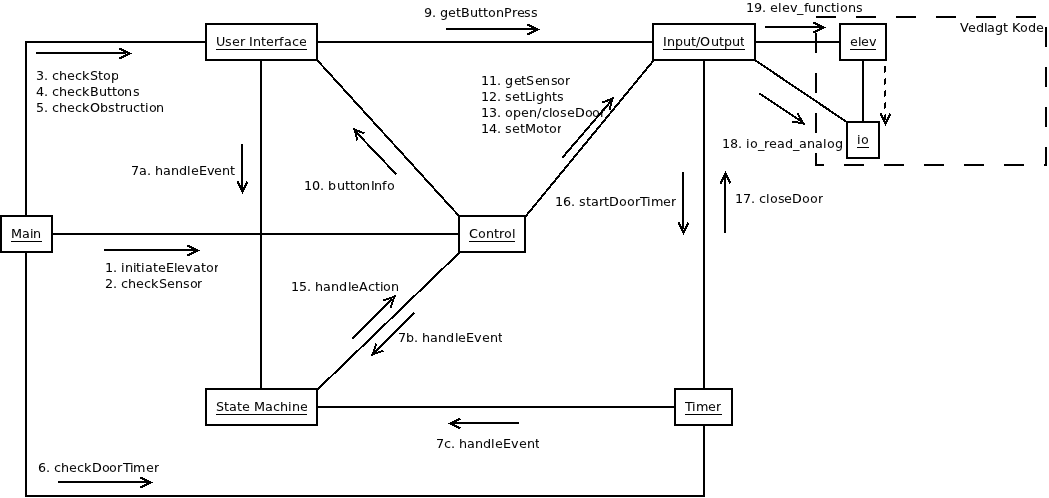
\includegraphics[width=\textwidth]{grafikk/systemarkitektur.png}
\caption{Overordnet systemarkitektur}
\end{figure}
\begin{description}
\item[1.] initiateElevator kalles hver gang heisprogrammet starter, og utf�rer oppstartsprosedyren beskrevet i Usecase-diagrammet.
\item[2. - 6.] check-funksjonene kalles kontinuerlig i main, og registrerer hendelser for tilstandsmaskinen.
\item[7.] handleEvent kalles av check-funksjonene i tre forskjellige klasser. HandleEvent kalles med et av argumentene NEW\_DESTINATION, FLOOR\_REACHED, STOP\_PRESSED og ORDER\_BUTTON\_PRESSED avhengig av hvilke hendelser check-funksjonene registrerer.
\item[8.] handleAction er et samlebegrep for handle-funksjonene som kalles av tilstandsmaskinen. 
\item[9.] betingelser er funksjoner som returnerer 0 eller 1. Disse m� v�re oppfylt (returnerer 1) for � f� en transisjon i tilstandsmaskinen der disse er satt som betingelse.
\item[10.] getUiSignals er et samlebegrep for funksjonene som henter signaler fra knappene og obstruksjon. Funksjonene kalles av check-funksjonene.
\item[11.] Siste bestillingsknapp som trykkes, lagres i ui-klassen, og getLastOrder returnerer denne til kontroll-klassen. 
\item[12.] getSensor er et samlebegrep for funksjoner som henter informasjon fra etasjesensorene. 
\item[13.] controlLights er et samlebegrep for funksjoner som skrur av og p� lys.
\item[14.] openDoor og closeDoor h�ndterer d�ra.
\item[15.] controlMotor er et samlebegrep for funksjoner som starter og stopper motoren.
\item[16.] startDoorTimer kalles n�r d�ra �pnes for � telle ned tre sekunder.
\item[17.] closeDoor kalles fra timer-klassen og lukker d�ra n�r timeren har telt ned.
\item[18.] io\_read\_analog er en funksjon som returnerer m�lt motorhastighet.
\item[19.] elevFunctions er funksjonene i det ferdige grensesnittet mot heisen.
\end{description}